
\documentclass[12pt,AutoFakeBold]{article} 

\usepackage[智能数据挖掘]{XDUreport}  % 科目名称
\problem{基于 $k$NN 的高光谱图像分类}  % 请在此处填写问题内容
% 其他参数在宏包中进行更改,其中学院,班级,姓名,学号均在sty宏包内进行更改
% \usepackage{fourier}  % 这是 fourier 字体,更柔和 

%% 如果你需要中文的一级标题编号,如“一、”、“二、”等,请把下面两行取消注释
% \RequirePackage{zhnumber} % change section number to chinese
% \titleformat{\section}{\Large\bfseries\rmfamily}{\zhnum{section}、}{0em}{}
%\usepackage[table,xcdraw]{xcolor}
%\definecolor{lightblue}{RGB}{222, 234, 246}

% 文档开始
        
\begin{document}

\maketitle
\setcounter{tocdepth}{2}

\tableofcontents  % 生成目录

% 正文标题
\makeatletter
\begin{center}
    \LARGE \textbf{\textsf{\@problem}}
\end{center}
\makeatother

% 正文开始

\section{数据集简介}

使用 Indian Pines 数据集,该数据集是由 AVIRIS 传感器在印第安纳州西北部的 Indian Pines 试验场上空采集的。图像大小为,共有 224 个光谱带。其空间分辨率为每像素 20 米。一般在实验中通过去除 4 个空带和 20 个损坏带,保留了 200 个光谱通道。该数据将共有 10249 个像素包含了真值信息,它们分别属于 16 个不同的类。

数据集地址: (数据集为.mat格式) \url{http://www.ehu.eus/ccwintco/index.php/Hyperspectral_Remote_Sensing_Scenes}(下载corrected Indian Pines和Indian Pines groundtruth)

\section{原理分析}

\subsection{$k$NN 方法}

$k$ 近邻($k$-Nearest Neighbor, $k$NN)学习是一种常用的监督学习方法,其工作原理:给定测试样本,基于某种距离度量找出训练集中与其最靠近的 $k$ 个训练样本,然后基于这 $k$ 个“邻居”的信息来进行预测。通常,在分类任务中可使用“投票法”,即选择这 $k$ 个样本中出现最多的类别标记作为预测结果;在回归任务中可使用“平均法”,即将这 $k$ 个样本的实值输出标记的平均值作为预测结果;还可基于距离远近进行加权平均或加权投票,距离越近的样本权重越大。分类中 $k$NN 的伪代码如算法 \ref{alg:KNN} 所示。

\begin{algorithm}[hbtp]
	\caption{$k$NN 方法}
	\label{alg:KNN}
	\begin{algorithmic}[1]
	\Require $\mathrm{X}$: 训练数据, $\mathrm{Y}$: $\mathrm{X}$ 的标签类, $x$: 未知数据;
	\Ensure $x$ 的预测类别; 
	
	\For{$x^{'}\in \mathrm{X}$}
		\State 计算距离 $d(x^{'},x)$;
	\EndFor
	\State 计算包含 $k$ 个最短距离 $d(X_i,x)$ 的下标集合 $I$;
	\\
	\Return 在 $I$ 中最多的标签类别 $Y_i$;
	\end{algorithmic} 
\end{algorithm}


\subsection{评价指标}

为了能够公正客观评价分类方法的表现,需要选取相应的评价指标。有四种常用的高光谱图像分类评价指标,分别为:总体分类精度 (Overall Accuracy,OA)、类别分类精度 (Class Accuracy,CA)、平均分类精度 (Average Accuracy,AA) 和 Kappa 系数。

假设 $N$ 为所有测试样本的总个数,通过将获得的分类结果图和地面真实图像相同位置进行对比可计算出混淆矩阵 $\mathrm{K}\in\mathbb{R}^{C\times C}$,其中 $C$ 表示样本的总类别数,且 $N=\sum_{i=1}^C\sum_{j=1}^C\mathrm{K}_{ij}$,$\mathrm{K}_{ij}$ 的值代表第 $i$ 类样本被划分成第 $j$ 类的样本数量。$\mathrm{OA}$ 代表分类结果与参考数据相吻合的概率,其计算公式为:
%
\begin{equation}
\mathrm{OA}=\frac{\displaystyle\sum_{i=1}^C\mathrm{K}_{ii}}{N}
\end{equation}
%
$\mathrm{CA}_i$ 代表第 $i$ 类样本被正确分类的概率,其计算公式为:
%
\begin{equation}
\mathrm{CA}_i=\frac{\mathrm{K}_{ii}}{\displaystyle\sum_{j=1}^C\mathrm{K}_{ij}}
\end{equation}
%
$\mathrm{AA}$ 代表各个类别分类精度的平均值,其计算公式为:
%
\begin{equation}
\mathrm{AA}=\frac{\displaystyle\sum_{i=1}^C\mathrm{CA}_i}{C}
\end{equation}
%
$\mathrm{Kappa}$ 系数是一种分类一致性评价指标,它在评价分类精度时还考虑了不确定性对分类结果造成的影响,其计算公式为:
%
\begin{equation}
\mathrm{Kappa}=\frac{N\displaystyle\sum_{i=1}^C\mathrm{K}_{ii}-\sum_{i=1}^C\left(\sum_{j=1}^C\mathrm{K}_{ij}\sum_{j=1}^C\mathrm{K}_{ji}\right)}{N^2-\displaystyle\sum_{i=1}^C\left(\sum_{j=1}^C\mathrm{K}_{ij}\sum_{j=1}^C\mathrm{K}_{ji}\right)}
\end{equation}
%

\section{实验过程}


\subsection{数据预处理}

通过 Python 中的 \lstinline[language=Python]|scipy.io.loadmat| 导入 Indian Pines 高光谱数据集并查看相关信息得到,数据集的形状为 $(145,145,200)$,ground truth 的形状是 $(145, 145)$,其中标签类别及数目如表 \ref{labelsnum} 所示,查看不同光谱下的图像示例如图 \ref{fig:diffband6} 所示。

\begin{figure}[hbtp]
	\centering
	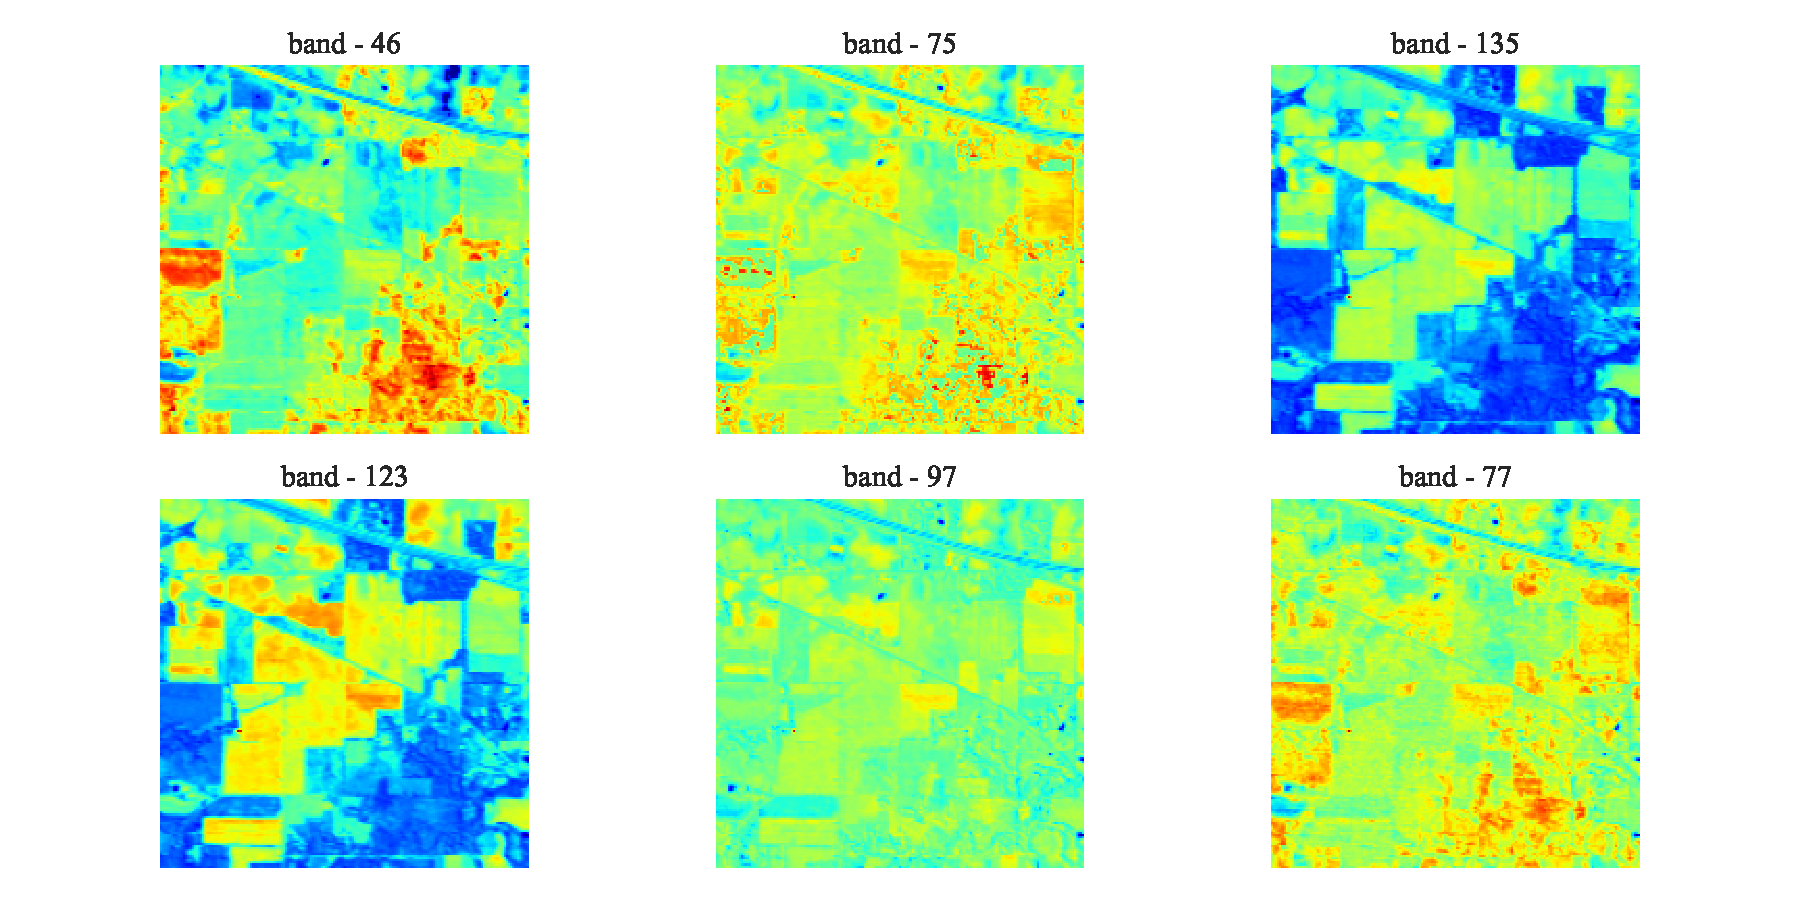
\includegraphics[width=16cm]{diffband6.pdf}
	\caption{不同光谱下的图像示例} \label{fig:diffband6}
\end{figure}

%\vspace{-0.5cm}
\begin{table}[h]
	\setlength{\abovecaptionskip}{0cm} 
	\setlength{\belowcaptionskip}{-0.2cm}
	\begin{center}
		\caption{标签类别及数目}
		\begin{tabular}{cccccccccccccccccc}
		\Xhline{4\arrayrulewidth}
		 0     & 11   & 2    & 14   & 10  & 3   & 6   & 12  & 5   & 8   & 15  & 4   & 13  & 16 & 1  & 7  & 9  \\
		\midrule[1pt]
		10776 & 2455 & 1428 & 1265 & 972 & 830 & 730 & 593 & 483 & 478 & 386 & 237 & 205 & 93 & 46 & 28 & 20 \\
		\Xhline{4\arrayrulewidth}
		\end{tabular} \label{labelsnum}
	\end{center}
\end{table}
\vspace{-0.6cm}

所有不同分类方法均采用 MIN-MAX 归一化预处理数据,数据集分割代码 \lstinline[language=Python]|train_test_split(pca, y, test_size=0.95, random_state=42, stratify=y)| 中的 \lstinline[language=Python]|stratify=y| 表示按每类比例分割,得到训练集标签类别及数目如表 \ref{testlabelsnum} 所示。

%\vspace{-0.5cm}
\begin{table}[h]
	\setlength{\abovecaptionskip}{0cm} 
	\setlength{\belowcaptionskip}{-0.2cm}
	\begin{center}
		\caption{训练集标签类别及数目}
		\begin{tabular}{cccccccccccccccccc}
		\Xhline{4\arrayrulewidth}
		 0     & 11   & 2    & 14   & 10  & 3   & 6   & 12  & 5   & 8   & 15  & 4   & 13  & 16 & 1  & 7  & 9  \\
		\midrule[1pt]
		539 & 123 & 71 & 63 & 49 & 41 & 37 & 30 & 24 & 24 & 19 & 12 & 10 & 5 & 2 & 1 & 1 \\
		\Xhline{4\arrayrulewidth}
		\end{tabular} \label{testlabelsnum}
	\end{center}
\end{table}
\vspace{-0.6cm}

\subsection{$k$NN 进行分类}

首先用 PCA 降成 $2\sim16$ 维等 15 个不同特征维度,每个不同特征维度 $k$NN 中 $k$ 取值为 $1\sim20$,得到不同特征维度的最好准确率如表 \ref{PCA_best} 所示,以及不同 $k$ 值下的准确率对比如图 \ref{fig:KNN_with_PCA} 所示,并且可以求出在特征维度为 8 且 $k=7$ 时有最大准确率 $0.645$。

%\vspace{-0.5cm}
\begin{table}[h]
	\setlength{\abovecaptionskip}{0cm} 
	\setlength{\belowcaptionskip}{-0.2cm}
	\begin{center}
		\caption{$k$NN 分类不同特征维度最好准确率}
		\begin{tabular}{cccccccc}
		\Xhline{4\arrayrulewidth}
		维度   & 2     & 3     & 4     & 5     & 6     & 7     & 8         \\ \hline
		准确率 & 0.588 & 0.629 & 0.627 & 0.635 & 0.642 & 0.642 & 0.643   \\ \midrule[1pt]
		9     & 10    & 11    & 12    & 13    & 14    & 15    & 16          \\ \hline
		0.639 & 0.637 & 0.637 & 0.638 & 0.640 & 0.640 & 0.640 & 0.640       \\
		\Xhline{4\arrayrulewidth}
		\end{tabular} \label{PCA_best}
	\end{center}
\end{table}
\vspace{-0.6cm}

\begin{figure}[htbp]
	\centering
	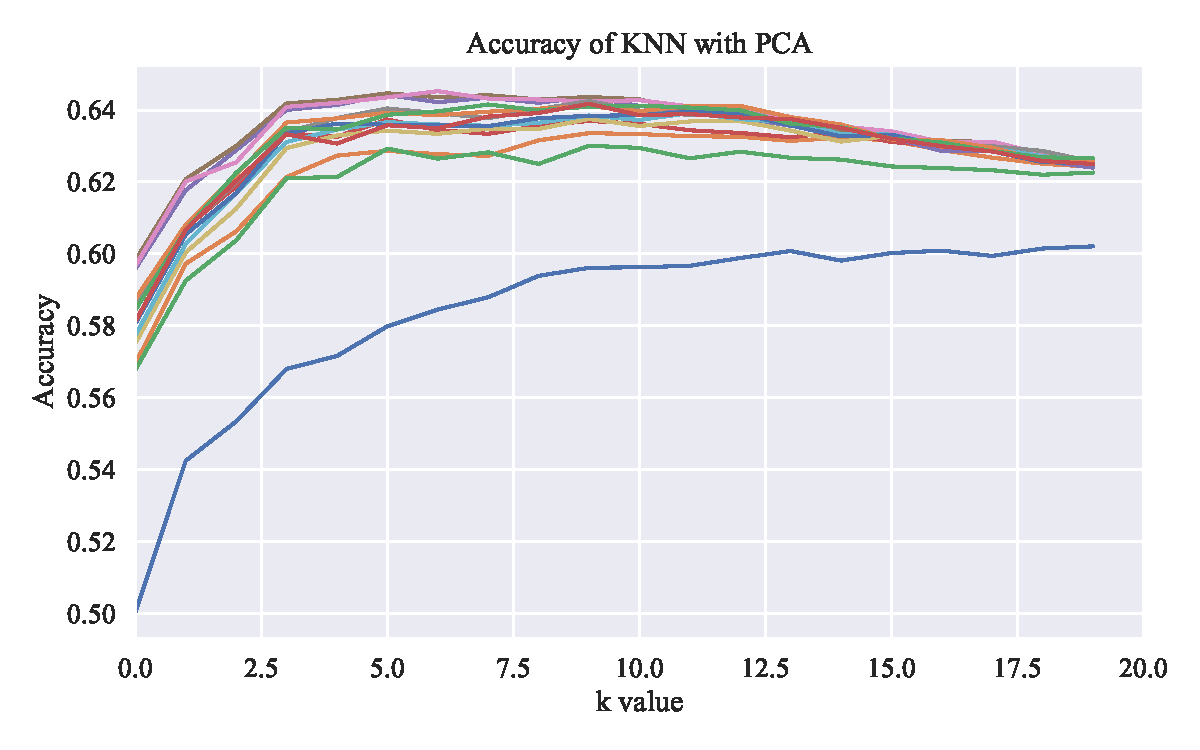
\includegraphics[width=0.7\textwidth]{KNN_with_PCA.pdf}
	\caption{$k$NN 方法不同 $k$ 值下的准确率} \label{fig:KNN_with_PCA}
\end{figure}

以最好的参数实验可以得到分类结果为 $\mathrm{OA}=0.645,\ \mathrm{AA}=0.352, \mathrm{kappa}=0.466$,$k$NN 分类结果图和 Ground Truth 分别如图 \ref{fig:KNN_Predict} 所示和图 \ref{fig:GT1} 所示。进行 10 折交叉验证可以得到准确率为 $0.670$。

\begin{figure}[htbp]
	\centering
	\begin{minipage}[t]{0.48\textwidth}
		\centering
		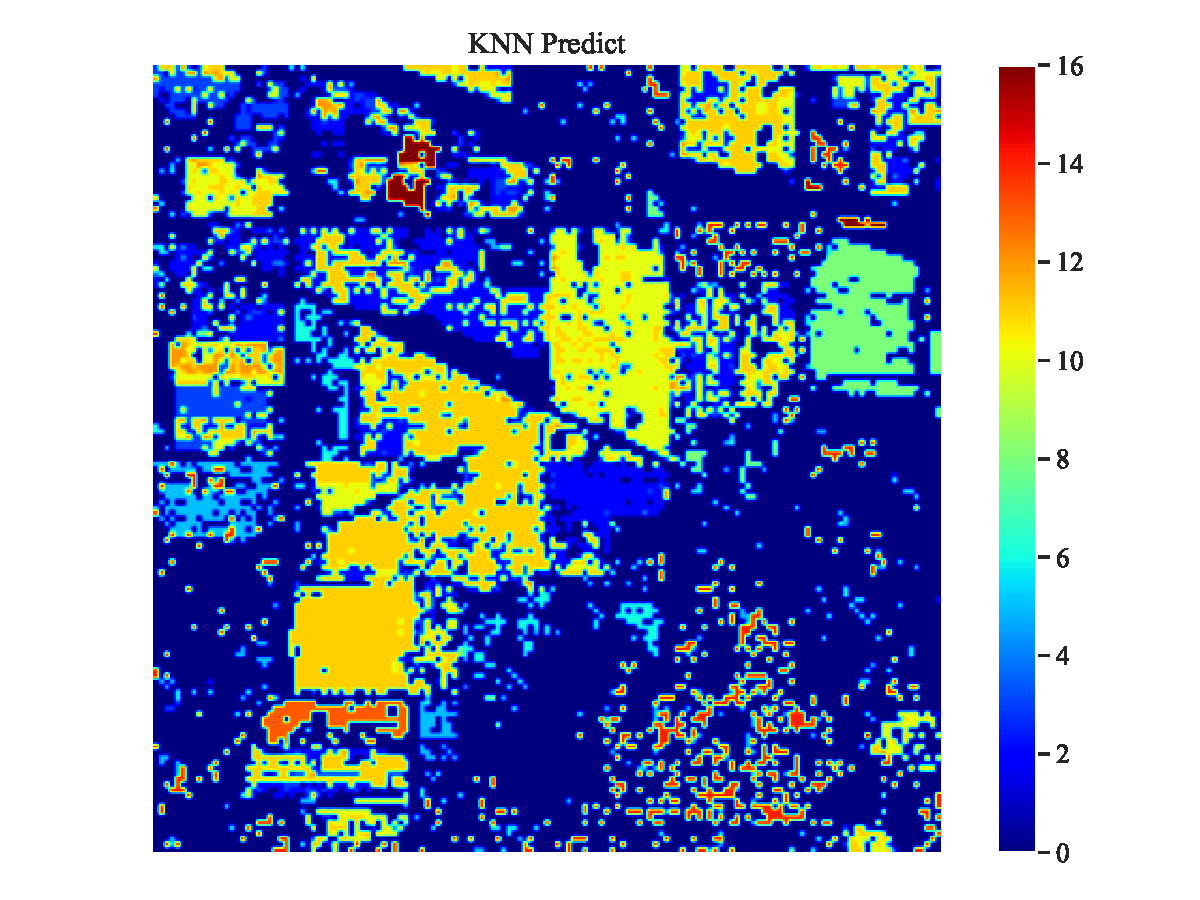
\includegraphics[height=7cm]{KNN_Predict.pdf}
		\caption{$k$NN 分类结果图} \label{fig:KNN_Predict}
	\end{minipage}
	\begin{minipage}[t]{0.48\textwidth}
		\centering
		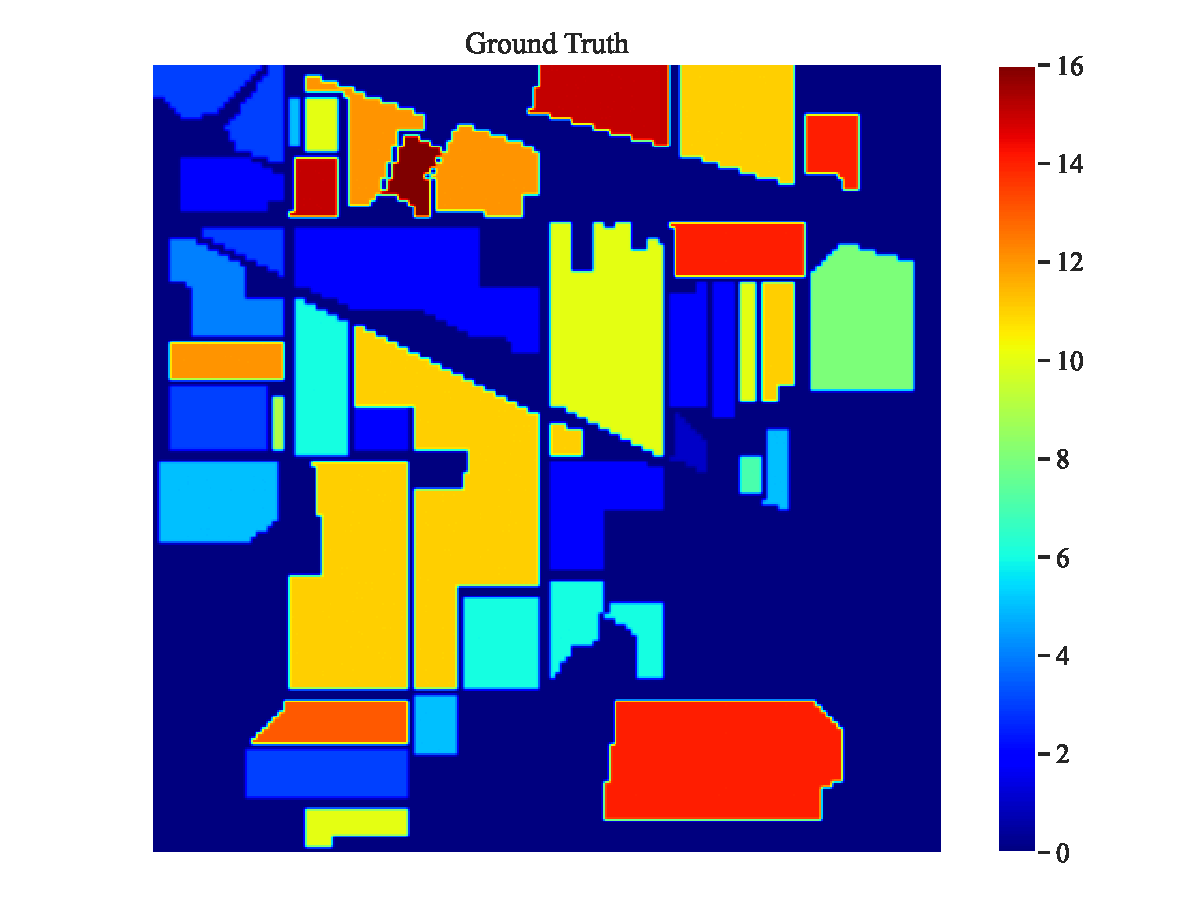
\includegraphics[height=7cm]{GT.pdf}
		\caption{Ground Truth} \label{fig:GT1}
	\end{minipage}
\end{figure}

$k$NN 分类得到的混淆矩阵和标准化后的混淆矩阵见附录。

\newpage

\includepdfset{pagecommand={\thispagestyle{fancy}}} 
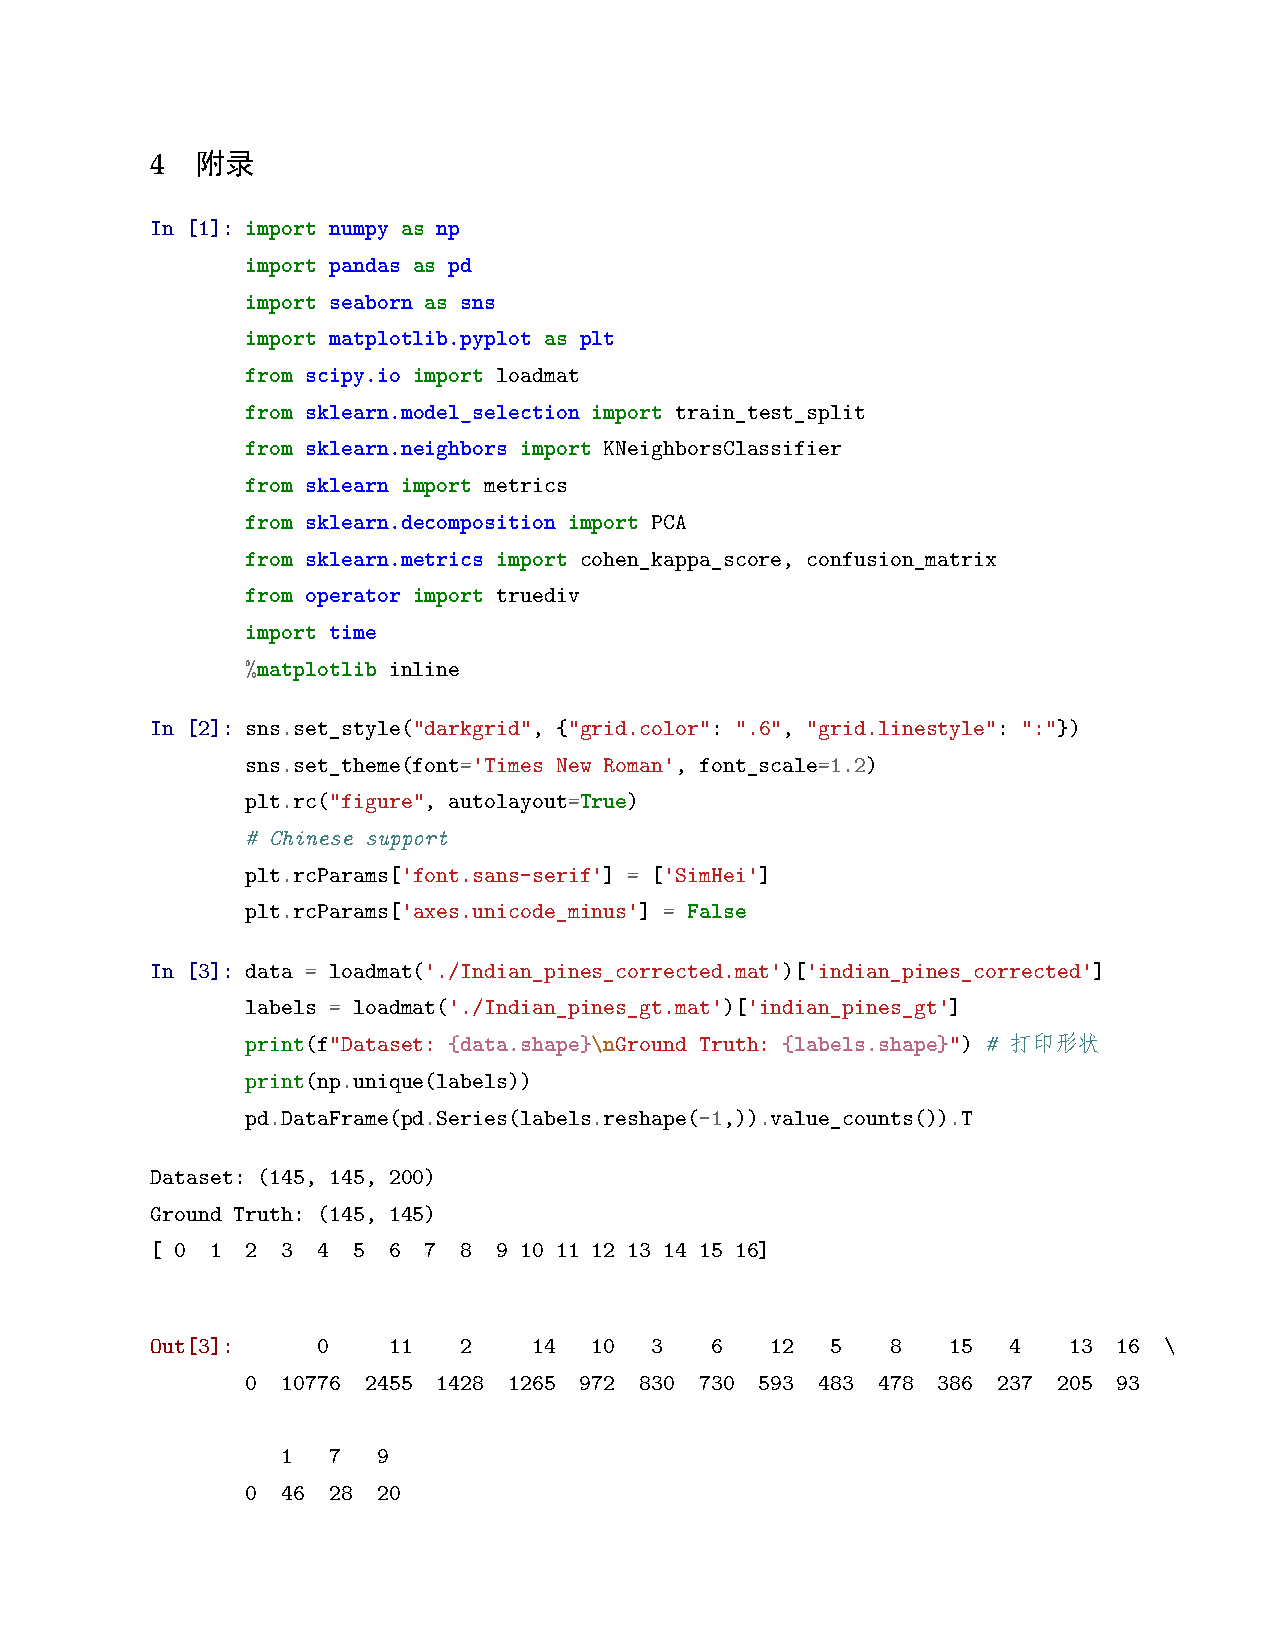
\includepdf[addtotoc={1,section,1,附录,appendix}, pages={1-14}]{KNN.pdf}

% % 参考文献,此处以 MLA 引用格式为例

% \begin{thebibliography}{9}
%     \bibitem{1} Clemente, Filipe Manuel, et al. "General network analysis of national soccer teams in FIFA World Cup 2014." \emph{International Journal of Performance Analysis in Sport} 15.1 (2015): 80-96.
%     \bibitem{3} Dijkstra, Edsger Wybe. "A Note on Two Problems in Connexion With Graphs." \emph{Numerische Mathematik} 1(1959):269-271.
%     \bibitem{4} Ahnert, Sebastian E., et al. "Ensemble approach to the analysis of weighted networks.." \emph{Physical Review E} 76.1 (2007).
%     \bibitem{5} Wong, J. A. Hartiganm. A. . "Algorithm AS 136: A K-Means Clustering Algorithm." \emph{Journal of the Royal Statistical Society. Series C (Applied Statistics)} 28.1(1979):100-108.
%     \bibitem{6} Buldu, J. M., et al. "Defining a historic football team: Using Network Science to analyze Guardiola’s F.C. Barcelona." \emph{Scientific Reports} 9.1 (2019): 1-14.
%     \bibitem{7} \emph{Balotelli sends Italy past Germany}. (2012). Retrieved December 10, 2014, from\url{https://www.uefa.com/uefaeuro/season=2012/matches/round=15174/match=2003379/index.html}
%     \bibitem{8} Sigari, Mohamad Hoseyn, et al. "Counterattack detection in broadcast soccer videos using camera motion estimation." \emph{international symposium on artificial intelligence} (2015): 101-106.
%     \bibitem{9} Abdelmahmoud Hassan Elsheikh. \emph{Effect of Leadership Intensity on Integrating Some Formal and Informal Organizational Efforts for Community Development in Khartoum Province}. 2016.
% \end{thebibliography}


% \includepdf[pages={1,2}]{Memo.pdf} 
% 可以直接导入pdf页面
% \newpage
% \begin{appendices}  % 附录环境
% \section{附录}
% \end{appendices}

\end{document}  % 结束